% ==============================================================================
% ================================== AUFGABE 2 ================================
% ==============================================================================

\section{Aufgabe 2: Feature Engineering -- Treibstoffverbrauch}
\label{sec:aufgabe2}

\subsection{Methodik}

Gemäß Aufgabenstellung werden die vier Aktionen auf Treibstoffkosten abgebildet: \emph{noop}~$=0$, \emph{left}~$=1$, \emph{main}~$=5$, \emph{right}~$=1$. Das Feature \texttt{fuel\_step} wird pro Schritt ergänzt, \texttt{fuel\_episode} als Summe pro Episode aggregiert. Das Vorgehen entspricht dem in KIPR00 beschriebenen Feature Engineering \cite[S.~23]{2}: Aus dem Domänenwissen über die Aktionen wird ein neues, aussagekräftigeres Merkmal konstruiert. Die Aggregation erfolgt mit den Standard-Pandas-Operationen \texttt{groupby} und \texttt{sum}, die Bibliothek wird bei Géron eingeführt \cite[S.~92]{1}.

\lstinputlisting[
    language=python,
    style=python,
    caption={Mapping der Aktionen auf Treibstoffkosten \textit{(eigene Darstellung)}},
    label={lst:fuel}
]{asset/code/Aufgabe2.py}

\subsection{Ergebnisse}

Die Validierung bestätigt, dass die Summe der Schritt-Fuel-Werte exakt der Summe der Episoden-Fuel-Werte entspricht (24\,268 Einheiten, eigene Berechnung). Der mittlere Treibstoffverbrauch pro Episode beträgt $485{,}36 \pm 28{,}04$ Einheiten (Min.~427, Max.~547). Die Top-5-Episoden nach Verbrauch erzielen Rewards zwischen $297{,}69$ und $312{,}33$, die Bottom-5-Episoden zwischen $261{,}77$ und $284{,}64$ (eigene Messung).

\begin{figure}[H]
    \centering
    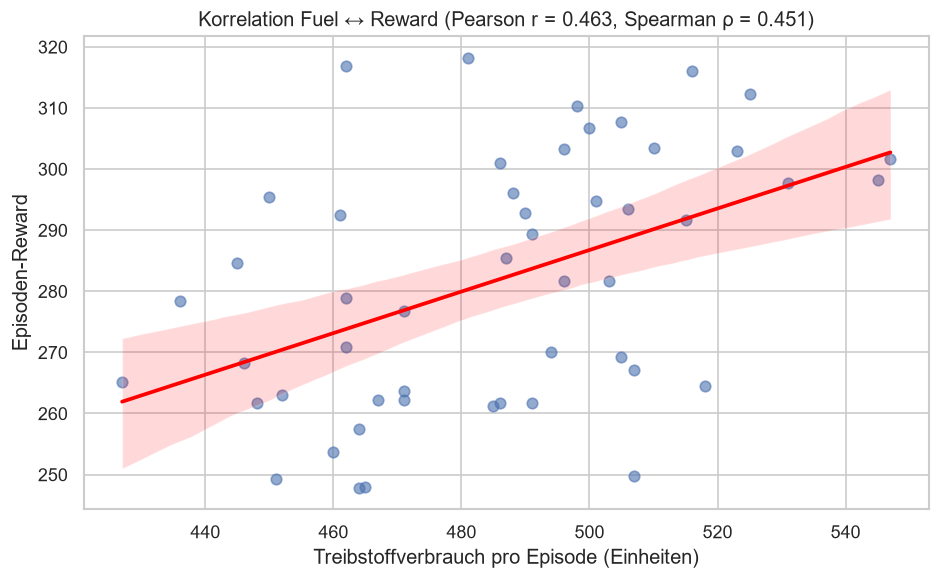
\includegraphics[width=1\linewidth]{asset/image/TomaKing_A2_Fuel_vs_Reward.png}
    \caption{Treibstoffverbrauch vs.\ Episoden-Reward \textit{(eigene Darstellung)}.}
    \label{fig:a2_fuel}
\end{figure}

\subsection{Interpretation}

Die Korrelation zwischen Treibstoff und Reward ist mit Pearson $r = 0{,}463$ (Spearman $\rho = 0{,}451$) moderat positiv (eigene Berechnung). Das Feature ist damit deutlich aussagekräftiger als die Episodenlänge ($r = 0{,}081$). Der positive Zusammenhang wird in Aufgabe~\ref{sec:aufgabe3} im Kontext der Reward-Struktur diskutiert. Die methodische Einordnung der Korrelationsstärke folgt den in KIPR00 beschriebenen Grundsätzen \cite[S.~22--23]{2}.

% ==============================================================================
% ================================== AUFGABE 2 ================================
% ==============================================================================